\addurlfn{event-emitter}{Event-Emitter}{https://nodejs.org/api/events.html}
\addurlfn{capacitor-electron-plattform}{Capacitor-Community Electron Plattform}{https://github.com/capacitor-community/electron}

\subsection{Zielsetzung}

Das Hauptziel des Capacitor-NodeJS Plugins ist die Entwicklung eines Plugins für Capacitor, welches es Entwicklern ermöglicht, Node.js Projekte in Capacitor Anwendungen zu integrieren.
Das Plugin soll eine \ac{api} bereitstellen, um zwischen der Node.js Runtime und der Anwendung zu kommunizieren.
Die \ac{api} soll an dem Node.js \fn{event-emitter} angelehnt werden, um die Kompatibilität mit vorhandenen Projekten zu verbessern.

\vspace{1em}

\begin{figure}[h]
    \centering
    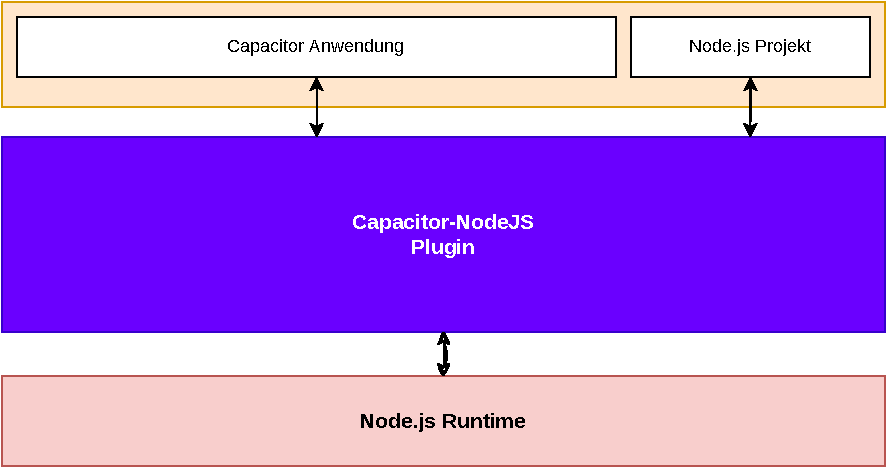
\includegraphics[width=\textwidth]{assets/02_Capacitor-NodeJS/01_Zielsetzung.drawio.pdf}
    \caption[Capacitor-NodeJS / Zielsetzung]{Zielsetzung des Capacitor-NodeJS Plugins}
\end{figure}

Als weiteres Ziel soll die Kompatibilität des Plugins mit der \fn{capacitor-electron-plattform} gewährleistet werden.
So soll das Plugin \textit{(und damit auch ein entsprechendes Node.js Projekt)} ohne zusätzlichen Aufwand sowohl in Mobile"=Anwendungen als auch in Desktop"=Anwendungen eingesetzt werden können.

\printfn
